\documentclass{exam}

\usepackage{indentfirst}
\usepackage{graphicx}
\usepackage{listings}
\usepackage{color}
\usepackage{fancyvrb}
\usepackage{amsmath}
\usepackage{amsfonts}
\usepackage{amssymb}
\usepackage{mathtools}
\usepackage{tkz-euclide}

\usetikzlibrary{angles,quotes,calc}

\definecolor{mygreen}{rgb}{0,0.6,0}
\definecolor{mygray}{rgb}{0.5,0.5,0.5}
\definecolor{mymauve}{rgb}{0.58,0,0.82}

\lstset{ %
	backgroundcolor=\color{white},		% choose the background color; you must add \usepackage{color} or \usepackage{xcolor}
	basicstyle=\small\ttfamily,		% the size of the fonts that are used for the code
	breakatwhitespace=false,			% sets if automatic breaks should only happen at whitespace
	breaklines=true,					% sets automatic line breaking
	captionpos=b,						% sets the caption-position to bottom
	columns=fullflexible,
	commentstyle=\color{mygreen},		% comment style
	deletekeywords={...},				% if you want to delete keywords from the given language
	escapeinside={\%*}{*)},			% if you want to add LaTeX within your code
	extendedchars=true,				% lets you use non-ASCII characters; for 8-bits encodings only, does not work with UTF-8
	frame=single,						% adds a frame around the code
	keepspaces=true,					% keeps spaces in text, useful for keeping indentation of code (possibly needs columns=flexible)
	keywordstyle=\color{blue},			% keyword style
	language=Octave,					% the language of the code
	morekeywords={*,...},				% if you want to add more keywords to the set
%   numbers=left,						% where to put the line-numbers; possible values are (none, left, right)
%   numbersep=6pt,						% how far the line-numbers are from the code
%   numberstyle=\tiny\color{mygray},	% the style that is used for the line-numbers
	rulecolor=\color{black},			% if not set, the frame-color may be changed on line-breaks within not-black text (e.g. comments (green here))
	showspaces=false,					% show spaces everywhere adding particular underscores; it overrides 'showstringspaces'
	showstringspaces=false,			% underline spaces within strings only
	showtabs=false,					% show tabs within strings adding particular underscores
	stepnumber=1,						% the step between two line-numbers. If it's 1, each line will be numbered
	stringstyle=\color{mymauve},		% string literal style
	tabsize=2,							% sets default tabsize to 2 spaces
	title=\lstname						% show the filename of files included with \lstinputlisting; also try caption instead of title
}

% Creates a new command to include a perl script, the first parameter is the filename of the script (without .pl), the second parameter is the caption
\newcommand{\octavescript}[2]{
\lstinputlisting[caption=#2,label=#1]{#1}
}

\newcommand{\MNLab}{Laborator\ \#3}
\newcommand{\MNLabTitle}{Ortogonalitate. Transformări ortogonale.}
\newcommand{\MNLabTitleHeader}{Ortogonalitate} 
\newcommand{\MNAuthor}{Andrei STAN, Mihaela-Andreea Vasile, Florin Pop}

\renewcommand{\contentsname}{Cuprins}
\renewcommand{\figurename}{Figura}
\renewcommand{\refname}{Referințe}

\setlength{\parskip}{0.5\baselineskip}

\graphicspath{{./img/}}

\title{
\textmd{\textbf{\MNLabTitle}}
\author{Colaboratori: \MNAuthor}
}

\pagestyle{headandfoot}

\header{Metode Numerice}
{\MNLabTitleHeader, Pagina \thepage\ din \numpages}
{2025}
\footer{Facultatea de Automatică și Calculatoare}{}{Pagina \thepage\ din \numpages}

\begin{document}

\begin{coverpages}

	\maketitle
	\tableofcontents

\end{coverpages}

\section{Obiective laborator}

\par În urma parcurgerii acestui laborator, studentul va fi capabil să:
\begin{itemize}
	\item definească noțiunile de vectori ortogonali și matrice ortogonală;
	\item aplice metode de transformare ortogonală: Householder și Givens;
	\item implementeze procesul Gram-Schmidt;
	\item folosească polinoame ortogonale.
\end{itemize}

\section{Noțiuni teoretice}

\subsection{Norme}

\par Considerând un spațiu vectorial $V$ peste un corp $\mathbb{K}$, o normă pe
$V$ este o funcție $||\cdot||: V \rightarrow \mathbb{R}$ care satisface
următoarele proprietăți pentru orice $x, y \in V$ și $\alpha \in \mathbb{K}$:

\begin{itemize}
	\item $||x|| \geq 0$ și $||x|| = 0 \Leftrightarrow x = 0$ (pozitiv definită);
	\item $||\alpha x|| = |\alpha| \cdot ||x||$;
	\item $||x + y|| \leq ||x|| + ||y||$ (inegalitatea triunghiului).
\end{itemize}

\subsubsection{Norme vectoriale}

\begin{itemize}
	\item \textbf{Valoarea absolută.} Este o normă pe $\mathbb{R}$ sau
	      $\mathbb{C}$. Numerele complexe formează un spațiu uni-dimensional
	      peste $\mathbb{C}$ și unul bi-dimensional peste $\mathbb{R}$.
	\item \textbf{Distanța Manhatten.} $||\mathbf{x}||_1 \coloneq \sum_{i} |x_i| $.
	\item \textbf{Norma euclidiană.} Pe $\mathbb{R}^n$, norma euclidiană este
	      definită ca $||\mathbf{x}||_2 \coloneq \sqrt{x_1^2 + x_2^2 + \ldots + x_n^2}$. Luând
	      în considerare numerele complexe, acestea se identifică cu $\mathbb{R}^2$.
	\item \textbf{Norma infinit.} $||\mathbf{x}||_{\infty} \coloneq \max_i |x_i|$.
	\item \textbf{Norma \textit{p}.} $||\mathbf{x}||_p \coloneq \left( \sum_{i} |x_i|^p \right)^{1/p}$.
	      Normele de mai sus sunt particularizări ale normei \textit{p} pentru diferite valori ale lui \textit{p}.

\end{itemize}

\subsubsection{Norme matriceale}

\par Multe norme matriceale mai au proprietatea de a fi \textit{submultiplicative}:

\begin{equation*}
	||AB|| \leq ||A|| \cdot ||B||
\end{equation*}

\begin{itemize}
	\item \textbf{Norma \textit{p} matriceală.} Ea este indusă de norma \textit{p} a vectorilor. \\
	      $||A||_p \coloneq \max_{x \neq 0} \frac{||Ax||_p}{||x||_p} = \max_{||x|| = 1} ||Ax||_p$.
	      \begin{itemize}
		      \item \textbf{p = 1.} $||A||_1 \coloneq \max_j \sum_i |a_{ij}|$. Este suma maximă a valorilor absolute
		            de pe coloane.
		      \item \textbf{p = 2. Norma/Raza spectrală.} $||A||_2 \coloneq \sqrt{\lambda_{max}(A^*A)}$.
		            Este rădăcina patrată a celei mai mari valori proprii a matricei $A^*A$.
		            Este egala cu cea mai mare valoare singulară a matricei $A$. \\
		            \textbf{Demonstrație.} Fie $B = A^*A$. Atunci $B$ este
		            simetrică și din teorema spectrală avem o bază ortonormată
		            de vectori proprii $v_i$ și valori proprii $\lambda_i$.
		            Fie $v = \sum_i \alpha_i v_i$ și $||v|| = 1$. Atunci:
		            \begin{equation*}
			            ||Av||^2_2 = \langle Av, Av \rangle = \langle v, A^*Av \rangle = \langle  \sum_{i} \alpha_i v_i, \sum_{i} \alpha_i \lambda_i v_i \rangle = \sum_{i} \lambda_i \alpha_i^2
		            \end{equation*}
		            Având constrângerea $||v|| = 1$, $\sum_{i} \alpha_i^2 = 1 \implies ||A||_2 = \lambda_{max}(A). \quad \blacksquare$

		      \item \textbf{p = $\infty$.} $||A||_{\infty} \coloneq \max_i \sum_j |a_{ij}|$. Este suma maximă a valorilor
		            absolute de pe rânduri.
	      \end{itemize}
	\item \textbf{Norma Frobenius.} $||A||_F \coloneq \sqrt{\sum_{i,j} |a_{ij}|^2} = \sqrt{trace(A^*A)}$.
\end{itemize}

\par \textbf{Teorema Gelfand.} Pentru orice normă matriceală avem:

\begin{equation*}
	\lim_{k \to \infty} ||A^k||^{1/k} = \rho(A)
\end{equation*}

\par Mai mult, $\rho(A) \leq ||A||$ pentru orice normă matriceală.

\par \textbf{Demonstrație.} Fie $\lambda$ valoarea proprie cea mai mare a lui $A$ și $v$ un vector propriu asociat. Atunci:

\begin{equation*}
	||A|| \geq \frac{||Av||}{||v||} (\forall v) = \frac{||\lambda v||}{||v||} = |\lambda| \Rightarrow \rho(A) \leq ||A||
\end{equation*}

\par Ce ne indică normele matriceale induse de vectori? Ele ne dau o măsură a
cât de mult se dilată un vector atunci când este aplicată o anumită transformare
liniară. În \ref{fig:1} avem o reprezentare a vectorilor unitari.

\begin{figure}[ht]
	\centering
	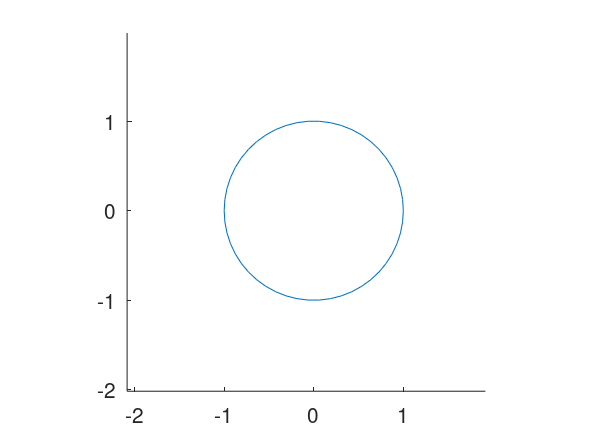
\includegraphics[width=0.5\textwidth]{plot1}
	\caption{Vectori unitate}
	\label{fig:1}
\end{figure}

\newpage
\par Ce se întâmplă dacă aplicăm transformarea $A1 = \begin{bmatrix} 3 & 2 \\ 1 & 4 \end{bmatrix}$?

\begin{figure}[ht]
	\centering
	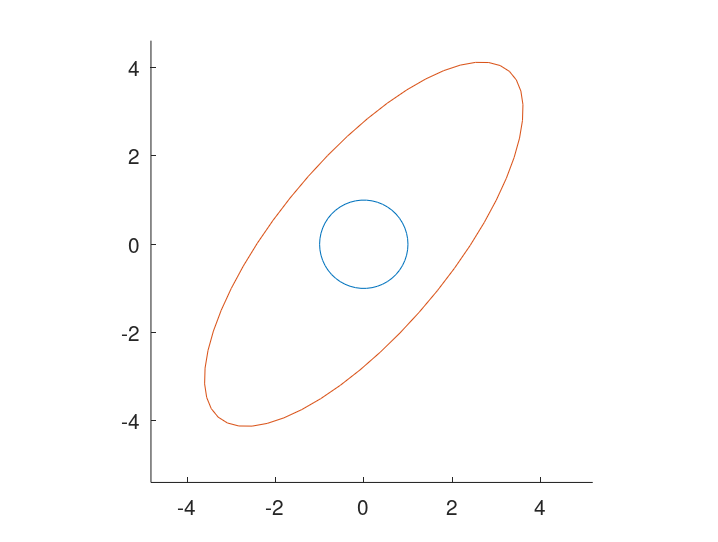
\includegraphics[width=0.5\textwidth]{plot2}
	\caption{Transformarea $A1$}
	\label{fig:2}
\end{figure}

\subsection{Produs scalar}

\par Produsul scalar al unui spațiu vectorial $V$ peste $F$ este o funcție
$\langle \cdot, \cdot \rangle: V \times V \rightarrow F$ care satisface
următoarele proprietăți pentru orice $x, y, z \in V$ și $\alpha \in F$:

\begin{itemize}
	\item $\langle x, y \rangle = \overline{\langle y, x \rangle}$ (conjugare simetrică);
	\item $\langle \alpha x + \beta y, z \rangle = \alpha \langle x, z \rangle + \beta \langle y, z \rangle$ (liniaritate);
	\item $\langle x, x \rangle \geq 0$ și $\langle x, x \rangle = 0 \Leftrightarrow x = 0$ (pozitivitate).
\end{itemize}

\par Din aceastea rezultă și altele:

\begin{itemize}
	\item $\langle x, \alpha y + \beta z \rangle = \overline{\alpha} \langle x, y \rangle + \overline{\beta} \langle x, z \rangle$;
	\item $\langle x + y, x + y \rangle = \langle x, x \rangle + 2 \Re(\langle x, y \rangle) +\langle y, y \rangle$;
\end{itemize}

\par Orice produs scalar induce o normă pe spațiul vectorial $V$ prin
$||x|| = \sqrt{\langle x, x \rangle}$.

\par Într-un spațiu euclidian, produsul
scalar este definit ca $\langle x, y \rangle = x^Ty$.

\subsubsection{Proiecții}

\par \textbf{Teoremă.} $\langle x, y \rangle = u^Tv = ||u||||v||\cos(\theta)$, unde $\theta$ este unghiul dintre cei doi vectori.

\par \textbf{Demonstrație.} Fie $\mathbf{r} = \mathbf{u} - \mathbf{v}$. Atunci,
din teorema cosinusului avem:

\begin{gather*}
	||\mathbf{r}||^2 = ||\mathbf{u}||^2 + ||\mathbf{v}||^2 - 2||\mathbf{u}||||\mathbf{v}||\cos(\theta) \\
	||\mathbf{u} - \mathbf{v}||^2 - ||\mathbf{u}||^2 - ||\mathbf{v}||^2 = -2||\mathbf{u}||||\mathbf{v}||\cos(\theta) \\
	-2 \sum_{i} u_iv_i = -2||\mathbf{u}||||\mathbf{v}||\cos(\theta) \\
	\sum_{i} u_iv_i = ||\mathbf{u}||||\mathbf{v}||\cos(\theta)
\end{gather*}

\par Astfel, putem scrie produsul scalar ca $\langle x, y \rangle = u^Tv = ||u||||v||\cos(\theta)$. $\blacksquare$

\par Fie doi vectori $\mathbf{x}$ și $\mathbf{y}$, iar proiecția lui $\mathbf{x}$
pe $\mathbf{y}$ este $\mathbf{x_y}$. Pentru a îl găsi pe $\mathbf{x_y}$, ne
gândim astfel:

\begin{itemize}
	\item În primul rând, ne trebuie norma lui $\mathbf{x_y}$: $||\mathbf{x}||\cos(\theta)$.
	\item Având norma, trebuie să avem și o direcție. Proiecția fiind pe $\mathbf{y}$,
	      o putem găsi prin \textit{normalizare}: $\frac{\mathbf{y}}{||\mathbf{y}||}$.
\end{itemize}

\begin{center}
	\begin{tikzpicture}[vect/.style={->,>={Straight Barb[angle=60:2pt 3]}}]
		\tkzInit[xmin=0,xmax=4,ymin=0,ymax=2]% dimensions of the bounding box
		\tkzDrawX[noticks,label=,draw=none]% coordinate system
		\tkzDrawY[noticks,label=,draw=none]
		\tkzDefPoint(0,0){O}
		\tkzDefPoint[label=$\mathbf{x}$](3,2){A}
		\tkzDefPoint[label=$\mathbf{y}$](4,0){B}
		\tkzDefPoint[label=$\mathbf{x_y}$](3,0){C}
		\tkzPointShowCoord[-,xlabel=$3$,ylabel=$4$,thin,gray,xstyle={below=4pt}](A)% show the coordonates
		\tkzPointShowCoord[-,xlabel=$6$,ylabel=$2$,thin,gray,xstyle={below=4pt}](B)
		\pic[draw, angle eccentricity=1.2, angle radius=1cm,, "$\theta$"] {angle=B--O--A};
		\tkzDrawSegments[vect](O,A O,B)
	\end{tikzpicture}
\end{center}

\par Avem și o interpretare geometrică a produsului scalar: produsul dintre
norma proiecției pe un vector și norma vectorului pe care se proiectează.

\par Definim operatorul de proiecție astfel: $proj_y x = \frac{||x|| \cos (\theta)}{||y||} y = \frac{\langle x, y \rangle}{\langle y, y \rangle} y$.

\begin{equation*}
	proj_y x = \frac{||x|| \cos (\theta)}{||y||} y = \frac{||y||||x|| \cos (\theta)}{||y||^2} y = \frac{\langle x, y \rangle}{\langle y, y \rangle} y
\end{equation*}

\subsection{Vectori ortogonali. Matrice unitară/ortogonală.}

\par Doi vectori $x, y \in \mathbb{R}^n$ sunt ortogonali dacă produsul lor
scalar este zero, adică $x^Ty = 0$. Cu alte cuvinte, direcțiile lor sunt
perpendiculare. În plus, dacă $||x||_2 = ||y||_2 = 1$, atunci cei doi
vectori sunt \textit{ortonormați}.

\par O bază a unui spațiu vectorial se numește ortogonală, respectiv ortonormată,
dacă vectorii acesteia sunt ortogonali, respectiv ortonormați.

\par O matrice $A \in \mathbb{C}^{n \times n}$ se numește \textit{unitară} dacă
$A^*A = AA^H = I_n$, unde $A^*$ este conjugata transpusă a lui $A$. Dacă $A$
este reală, atunci matricea se numește \textit{ortogonală} și putem scrie
$A^TA = AA^T = I_n$. Ele sunt foarte utilizate în diverse aplicații, precum
descompunerea QR sau descompunerea valorilor singulare.

\par O matrice $A \in \mathbb{C}^{n \times n}$ sau $\mathbb{R}^{n \times n}$
unitară/ortogonală are următoarele proprietăți:

\begin{itemize}
	\item coloanele (rândurile) sale formează o bază ortonormată a spațiului
	      vectorial $\mathbb{C}^n$ sau $\mathbb{R}^n$;
	\item norma vectorilor coloană (rând) este 1;
	\item $A^{-1} = A^*$ sau $A^{-1} = A^*$;
	\item este normală, adică $A^*A = AA^*$;
	\item este diagonalizabilă;
	\item valorile proprii se află pe cercul unitate;
	\item vectorii proprii sunt ortogonali;
	\item $det(A) = \pm 1$;
	\item $||A||_2 = 1$;
	\item conservă produsul scalar: $(Ax)^*(Ay) = x^*A^*Ay = x^*y$;
\end{itemize}

\par Astfel, matricile ortogonale se pot interpreta geometric ca fiind rotații,
reflecții, permutări, identități sau combinații ale acestora.

\par Ce se întâmplă dacă aplicăm o matrice ortogonală asupra vectorilor unitari? \\
Fie $A2 = \begin{bmatrix} \cos(\frac{\pi}{7}) & -sin(\frac{\pi}{7}) \\ sin(\frac{\pi}{7}) & cos(\frac{\pi}{7}) \end{bmatrix}$.

\begin{figure}[ht]
	\centering
	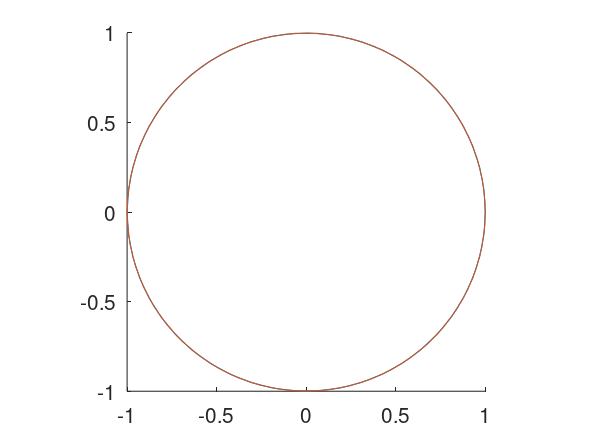
\includegraphics[width=0.5\textwidth]{plot3}
	\caption{Transformarea $A2$}
	\label{fig:3}
\end{figure}

\newpage
\par Toți vectorii au fost rotiți cu un unghi de $\frac{\pi}{7}$. Nu s-a
modificat nimic altceva! Norma vectorilor a rămas la fel și deci graficele
coincid. În următoarea figură, aplicăm $A3 = 2 * A2$, matrice care nu mai este
ortogonală.

\begin{figure}[ht]
	\centering
	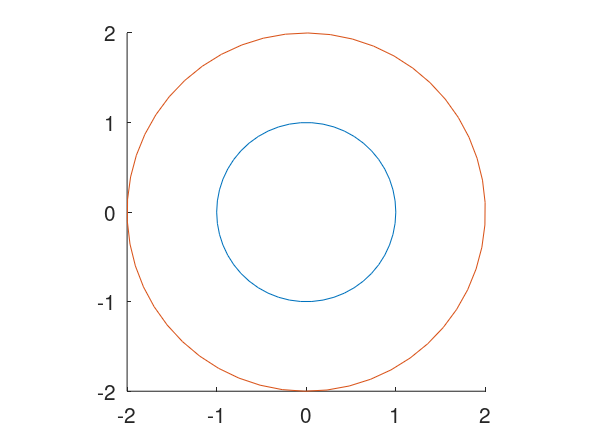
\includegraphics[width=0.5\textwidth]{plot4}
	\caption{Transformarea $A2$}
	\label{fig:4}
\end{figure}

\subsection{Transformări ortogonale. Descompunerea QR.}

\par \textbf{Definiție.} Fie $T: V \rightarrow V$ o transformare liniară.

\begin{equation*}
	T \text{ - ortogonală} \equiv \langle T(x), T(y) \rangle = \langle x, y \rangle
\end{equation*}

\par Utilitatea transformărilor ortogonale în cazul sistemelor liniare constă în
faptul că putem aplica o serie de astfel transformări pentru a introduce 0-uri
în matricea sistemului. La final, aflarea soluției va consta în rezolvarea unui
sistem triunghiular. Matricea va avea forma $A = QR$, unde $Q$ este o matrice
ortogonală și $R$ este o matrice superior triunghiulară.

\begin{equation*}
	Ax = b \Leftrightarrow QRx = b \Leftrightarrow Rx = Q^*b
\end{equation*}

\par Cu aceste transformări, ne dorim să aducem vectori de la forma
$\begin{bmatrix} x \\ y \end{bmatrix}$ la forma $\begin{bmatrix} x' \\ 0 \end{bmatrix}$.

\subsubsection{Reflexii. Transformarea Householder.}

\par Căutăm o transformare $P$ astfel încât $P v = ||v|| e$, unde $e$ este un
vector din baza canonică.

\par Pentru reflexie, ne alegem un vector $d$ care ne va da
\textit{direcția de reflexie}, $||d||_2 = 1$

\begin{center}
	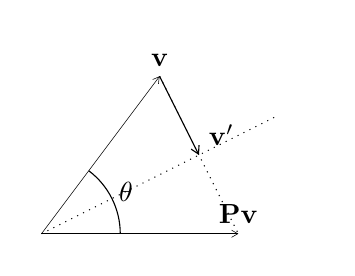
\begin{tikzpicture}[vect/.style={->,>={Straight Barb[angle=60:2pt 3]}}]
		\tkzInit[xmin=0,xmax=3,ymin=0,ymax=2]% dimensions of the bounding box
		\tkzDrawX[noticks,label=,draw=none]% coordinate system
		\tkzDrawY[noticks,label=,draw=none]

		\tkzDefPoint(0,0){O}
		\tkzDefPoint[label=$\mathbf{v}$](1.5,2){A}
		\tkzDefPoint[label=$\mathbf{P v}$](2.5,0){B}

		\tkzDefMidPoint(A,B) \tkzGetPoint{M}
		\tkzGetPointCoord(M){Mx,My}
		\coordinate (Bisector) at ($(O)!1.5!(M)$);

		\draw[dotted] (O) -- (Bisector);
		\draw[dotted] (A) -- (B);
		\draw[vect] (A) -- (M) node[above right] {$\mathbf{v'}$};

		\pic[draw, angle eccentricity=1.2, angle radius=1cm, "$\theta$"] {angle=B--O--A};
		\tkzDrawSegments[vect](O,A O,B)
	\end{tikzpicture}
\end{center}

\begin{align*}
	v' & = proj_d (-v) = \frac{\langle v, d \rangle}{\langle d, d \rangle} d \\
	v' & = - v^* d d = - d d^* v \implies
\end{align*}
\begin{align*}
	P v & = v - 2 v' = v - 2 d d^* v \\
	P   & = I - 2 d d^*
\end{align*}

\par Iar în cazul în care $d$ nu are norma 1, ajungem la forma generală a
reflectorului Householder, prin normalizare:

\begin{equation*}
	P = I - 2 \frac{d d^T}{d^T d}
\end{equation*}

\par \textbf{Afirmație.} $P$ este ortogonală.

\par \textbf{Demonstrație.} $P^TP = (I - 2 d d^*)^*(I - 2 d d^*) = I - 2 d d^* - 2 d d^* + 4 d d^* d d^* = I - 4 d d^* + 4 d d^* = I$. $\blacksquare$

\par \textbf{Cum găsim $d$ pentru a introduce 0-uri?}

\par Cum $P$ este ortognală, știm că $||Pv||_2 = ||v||_2$. Astfel, ne dorim ca $Pv = \pm ||v||_2 e_1$.

\begin{align*}
	v + d & = P v                                                                        \\
	v + d & = \pm ||v||_2 e_1                                                            \\
	d     & = \pm ||v||_2 e_1 - v, \text{cum semnul lui } d \text{ nu contează, alegem } \\
	d     & = v \pm ||v||_2 e_1
\end{align*}

\par \textbf{Plus sau minus?} Răspunsul îl putem găsi efectuând puțină analiză
numerică, fără a demonstra nimic formal de data asta. Plecăm de la următoarea
întrebare: Este bine ca $Pv$ și $v$ să fie apropiate?

\par Știind că calculul numeric nu este perfect, putem presupune că nici
reflexia nu va fi perfectă. Problema este că dacă $\mathbf{v}$ este deja foarte
aproape de axe, e foarte posibil ca $\mathbf{Pv}$ să fie chiar mai departe de
aceasta.

\par În schimb, dacă $\mathbf{v}$ și reflexia acestuia sunt depărtate,
eroare poate fi neglijabilă.

\par Ne dorim ca $||v - \alpha ||v||_2 e_1||_2$ să fie maximă, unde
$\alpha = \pm 1$. Considerăm doar cazul numerelor reale.

\begin{align*}
	||v - \alpha ||v||_2||_2 = (v - \alpha ||v||_2 e_1)^T (v - \alpha ||v||_2 e_1) & = (v - \alpha ||v||_2 e_1)^T(v - \alpha ||v||_2 e_1)           \\
	                                                                               & = v^Tv - 2 \alpha ||v||_2 v^Te_1 + \alpha^2 ||v||_2^2 e_1^Te_1 \\
	                                                                               & = v^Tv - 2 \alpha ||v||_2 v_1 + ||v||_2^2
\end{align*}

\par Cum $v^Tv$ și $||v||_2^2$ sunt constante, trebuie să găsim maximul
termenului $- \alpha ||v||_2 v_1$, mai precis $- \alpha v_1$. Cum $\alpha$ poate fi
doar 0 sau 1, rezultă imediat că $\alpha = -sign(v_1)$.

\newpage
\par În figura de mai jos (figura \ref{fig:5}), avem un grafic al
$||A - QR||_2 / ||A||_2$. Au fost generate 1000 de teste, deci avem 1000 de puncte pe
grafic. În fiecare test s-a generat o matrice 3x3 aleatorie iar prima sa coloană
a fost înlocuită cu $\begin{bmatrix} 1 & \delta & 0 \end{bmatrix}^T$, unde
$\delta$ lua 17 valori între $10^{-16}$ și $1$. Cu albastru avem cazul când
alegem semnul ca mai sus, iar cu roșu când alegem semnul opus.

\begin{figure}[ht]
	\centering
	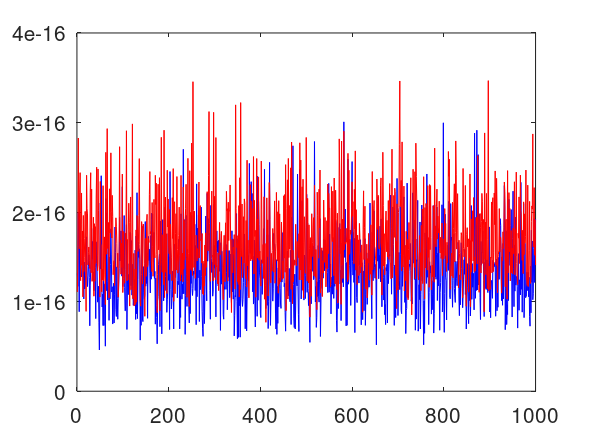
\includegraphics[width=0.5\textwidth]{hbad}
	\caption{Eroarea relativă}
	\label{fig:5}
\end{figure}

\par Se poate observa că eroarea relativă, în medie, mai mică atunci când alegem
semnul bine.

\par \textbf{Anulare catastrofală.} Având o precizie limitată în calculul
numeric, se pare că diferența a două aproximari a unor numere foarte apropiate
poate duce la o aproximare foarte rea.

\par \textbf{Demonstrație.} Fie aproximările $\overline{x}$ și $\overline{y}$,
cu erorile relative $\epsilon_x = \frac{x - \overline{x}}{x}$ și $\epsilon_y = \frac{y - \overline{y}}{y}$.

\begin{align*}
	\overline{x} & = x(1 + \epsilon_x) \\
	\overline{y} & = y(1 + \epsilon_y)
\end{align*}

\par Atunci,

\begin{align*}
	\overline{x} - \overline{y} & = x(1 + \epsilon_x) - y(1 + \epsilon_y) = x - y + x \epsilon_x - y \epsilon_y                           \\
	                            & = x - y + (x - y) \epsilon_{xy}, \text{unde } \epsilon_{xy} = \frac{x \epsilon_x - y \epsilon_y}{x - y} \\
	                            & = (x - y)(1 + \epsilon_{xy})
\end{align*}

\par Numitorul lui $\epsilon_{xy}$ este foarte mic daca $x \approx y$, deci
eroarea devine foarte mare. $\blacksquare$

\par În concluzie, obținem următoarea formulă pentru $d$: $d = v + sign(v_1) ||v||_2 e_1$.

\par Pentru a oferi un exemplu practic a descompunerii QR cu Householder, mai
e utilă următoarea informație: putem "umple" vectorul $d$ cu 0-uri în locurile
unde ne dorim ca vectorii să nu fie afectați. De exmeplu, dacă avem 3 dimensiuni
și vrem să punem 0 \textbf{doar} pe poziția 3, atunci $d = \begin{bmatrix} 0 \\ v2 - sign(v_2) ||v'||_2 \\ v3 \end{bmatrix}$
sau $d = \begin{bmatrix} v1 - sign(v_1) ||v'||_2 \\ 0 \\ v3 \end{bmatrix}$, unde $v' = \begin{bmatrix} v2 \\ v3 \end{bmatrix}$,
respectiv $v' = \begin{bmatrix} v1 \\ v3 \end{bmatrix}$

\par \textbf{Exemplu.} Fie matricea $A_1 = \begin{bmatrix} 2 & 4 & 5 \\ 1 & -1 & 1 \\ 2 & 1 & -1 \end{bmatrix}$.
Ne dorim să găsim matricea $Q$ și $R$ astfel încât $A = QR$ și $Q$ să fie ortogonală.

\par La prima iterație ne dorim să punem 0-uri pe pozițiile (2, 1) și (3, 1).

\begin{equation*}
	v = \begin{bmatrix} 2 \\ 1 \\ 2 \end{bmatrix}, \quad ||v||_2 = 3, \quad d = \begin{bmatrix} 2 -sign(2) * 3 \\ 1 \\ 2 \end{bmatrix} = \begin{bmatrix} -1 \\ 1 \\ 2 \end{bmatrix}, \quad ||d||_2^2 = 6
\end{equation*}

\begin{align*}
	H_1           & = I_3 - 2 \frac{d d^T}{d^T d} = \begin{bmatrix} 1 & 0 & 0 \\ 0 & 1 & 0 \\ 0 & 0 & 1 \end{bmatrix} - \frac{1}{3} \begin{bmatrix} -1 \\ 1 \\ 2 \end{bmatrix} \begin{bmatrix} -1 & 1 & 2 \end{bmatrix}                                        \\
	H_1           & = \begin{bmatrix} 1 & 0 & 0 \\ 0 & 1 & 0 \\ 0 & 0 & 1 \end{bmatrix} - \frac{1}{3} \begin{bmatrix} 1 & -1 & -2 \\ -1 & 1 & 2 \\ -2 & 2 & 4 \end{bmatrix} = \frac{1}{3} \begin{bmatrix} 2 & 1 & 2 \\ 1 & 2 & -2 \\ 2 & -2 & -1 \end{bmatrix} \\
	A_2 = H_1 A_1 & = \frac{1}{3} \begin{bmatrix} 2 & 1 & 2 \\ 1 & 2 & -2 \\ 2 & -2 & -1 \end{bmatrix} \begin{bmatrix} 2 & 4 & 5 \\ 1 & -1 & 1 \\ 2 & 1 & -1 \end{bmatrix} = \begin{bmatrix} 3 & 3 & 3 \\ 0 & 0 & 3 \\ 0 & 3 & 3 \end{bmatrix}
\end{align*}

\par La a doua iterație ne dorim să punem 0 pe poziția (2, 3).

\begin{equation*}
	v = \begin{bmatrix} 0 \\ 3 \end{bmatrix}, \quad ||v||_2 = 3, \quad d = \begin{bmatrix} 0 \\ -sign(0) * 3 \\ 3 \end{bmatrix} = \begin{bmatrix} 0 \\ -3 \\ 3 \end{bmatrix}, \quad ||d||_2^2 = 18
\end{equation*}

\begin{align*}
	H_2           & = I_3 - 2 \frac{d d^T}{d^T d} = \begin{bmatrix} 1 & 0 & 0 \\ 0 & 1 & 0 \\ 0 & 0 & 1 \end{bmatrix} - \frac{1}{9} \begin{bmatrix} 0 \\ -3 \\ 3 \end{bmatrix} \begin{bmatrix} 0 & -3 & 3 \end{bmatrix}                         \\
	H_2           & = \begin{bmatrix} 1 & 0 & 0 \\ 0 & 1 & 0 \\ 0 & 0 & 1 \end{bmatrix} - \frac{1}{9} \begin{bmatrix} 0 & 0 & 0 \\ 0 & 9 & -9 \\ 0 & -9 & 9 \end{bmatrix} = \begin{bmatrix} 1 & 0 & 0 \\ 0 & 0 & -1 \\ 0 & -1 & 0 \end{bmatrix} \\
	A_3 = H_2 A_2 & = \begin{bmatrix} 1 & 0 & 0 \\ 0 & 0 & -1 \\ 0 & -1 & 0 \end{bmatrix} \begin{bmatrix} 3 & 3 & 3 \\ 0 & 0 & 3 \\ 0 & 3 & 3 \end{bmatrix} = \begin{bmatrix} 3 & 3 & 3 \\ 0 & -3 & -3 \\ 0 & 0 & -3 \end{bmatrix}
\end{align*}

\par $A_3$ este matricea $R$, iar $Q = H_1^T H_2^T = H_1 H_2$ este matricea ortogonală.

\subsubsection{Rotații Givens}

\par Pentru demonstrarea acestor rotiri ne putem referi foarte simplu la numerele
complexe. Fără a demonstra, putem identifica orice număr complex de forma $a + bi$
ca fiind un vector din $\mathbb{R}^2$, $\begin{bmatrix} a \\ b \end{bmatrix}$.
Înmulțirea acestui număr cu un alt număr complex $c + di$ este echivalentă cu
înmulțirea vectorului cu matricea $\begin{bmatrix} c & -d \\ d & c \end{bmatrix}$.

\par Știind că $ (\cos \alpha + i \sin \alpha)(\cos \beta + i \sin \beta) = \cos(\alpha + \beta) + i \sin(\alpha + \beta)$,
și că orice număr complex poate fi scris sub forma $r(\cos \beta + i \sin \beta)$,
putem deduce că înmulțirea cu matricea $\begin{bmatrix} \cos \theta & -\sin \theta \\ \sin \theta & \cos \theta \end{bmatrix}$
rotește vectorii cu un unghi $\theta$, în sens trigonometric. Această matrice
este una ortognală.

\begin{equation*}
	\begin{bmatrix} \cos \theta & \sin \theta \\ -\sin \theta & \cos \theta \end{bmatrix} \begin{bmatrix} \cos \theta & -\sin \theta \\ \sin \theta & \cos \theta \end{bmatrix} = I
\end{equation*}

Cum $-\sin \theta = \sin(-\theta)$, putem vedea prima matrice din ecuația de mai
sus ca o rotație cu $-\theta$.

\par Prin aceste rotații, ne dorim același lucru ca și la Householder, să aducem
vectori de la forma $\begin{bmatrix} x \\ y \end{bmatrix}$ la forma
$\begin{bmatrix} x' \\ 0 \end{bmatrix}$. Fiind o transformare ortogonală, norma
vectorilor se păstrează și am avea că $x' = \sqrt{x^2 + y^2}$. Pentru a calcula
matricea, nu avem nevoie de unghi, ci doar de $\cos$ și $\sin$.

\begin{equation*}
	\begin{bmatrix} \cos \theta & -\sin \theta \\ \sin \theta & \cos \theta \end{bmatrix} \begin{bmatrix} x \\ y \end{bmatrix}
	= \begin{bmatrix} x \cos \theta - y \sin \theta \\ y \cos \theta + x \sin \theta \end{bmatrix}
	= \begin{bmatrix} \sqrt{x^2 + y^2} \\ 0 \end{bmatrix}
\end{equation*}

\par Rezolvând acest sistem găsim că $\cos \theta = \frac{x}{\sqrt{x^2 + y^2}}$ și
$\sin \theta = - \frac{y}{\sqrt{x^2 + y^2}}$.

\par Pentru matrici mai mari, de dorim să găsim o matrice $G$ astfel încât

\begin{equation*}
	G \begin{bmatrix} a \\ \vdots \\ x \\ \vdots \\ y \\ \vdots \\ z \end{bmatrix} = \begin{bmatrix} a \\ \vdots \\ x' \\ \vdots \\ 0 \\ \vdots \\ z \end{bmatrix}
\end{equation*}

\par $G$ seamănă foarte mult cu matricea identitate și se numește matricea Givens.

\begin{equation*}
	G =
	\begin{bmatrix}   1      & \cdots & 0      & \cdots & 0      & \cdots & 0      \\
                  \vdots & \ddots & \vdots &        & \vdots &        & \vdots \\
                  0      & \cdots & c      & \cdots & -s     & \cdots & 0      \\
                  \vdots &        & \vdots & \ddots & \vdots &        & \vdots \\
                  0      & \cdots & s      & \cdots & c      & \cdots & 0      \\
                  \vdots &        & \vdots &        & \vdots & \ddots & \vdots \\
                  0      & \cdots & 0      & \cdots & 0      & \cdots & 1
	\end{bmatrix}
\end{equation*}

\par Cu alte cuvinte, matricea $G$ este plină de 0 mai puțin următoarele
elemente: $G(i, i) = G(j, j) = c$, $G(i, j) = s$ și $G(j, i) = -s$, unde $i$
și $j$ sunt pozițiile pe care se găsește $y$, respectiv $x$. Asta înseamnă că $i$
va indica mereu poziția elementului în vector pe care vrem să îl facem 0.
O regulă bună la descompunerea QR este ca $(i, j)$ să fie fix poziția
elementului din matrice pe care vrem sa îl facem 0.

\par \textbf{Exemplu.} Fie $A_1 = \begin{bmatrix}
		0 & 1 & 2 \\
		3 & 2 & 0 \\
		4 & 1 & 5
	\end{bmatrix}$. Ne dorim să găsim matricea $Q$ și $R$ astfel încât $A = QR$ și $Q$ să fie ortogonală.

\par Facem 0 pe poziția $(3, 1)$.

\begin{equation*}
	(i, j) = (3, 1), \quad x = 0, \quad y = 4, \quad r = \sqrt{0^2 + 4^2} = 4, \quad c = \frac{x}{r} = 0, \quad s = -\frac{y}{r} = -1
\end{equation*}

\begin{align*}
	G_1           & = \begin{bmatrix}
		                  0  & 0 & 1 \\
		                  0  & 1 & 0 \\
		                  -1 & 0 & 0
	                  \end{bmatrix} \\
	A_2 = G_1 A_1 & = \begin{bmatrix}
		                  4 & 1  & 5  \\
		                  3 & 2  & 0  \\
		                  0 & -1 & -2
	                  \end{bmatrix}
\end{align*}

\par Facem 0 pe poziția $(2, 1)$.

\begin{equation*}
	(i, j) = (2, 1), \quad x = 4, \quad y = 3, \quad r = \sqrt{4^2 + 3^2} = 5, \quad c = \frac{x}{r} = \frac{4}{5}, \quad s = -\frac{y}{r} = -\frac{3}{5}
\end{equation*}

\begin{align*}
	G_2           & = \begin{bmatrix}
		                  \frac{4}{5}  & 0 & \frac{3}{5} \\
		                  0            & 1 & 0           \\
		                  -\frac{3}{5} & 0 & \frac{4}{5}
	                  \end{bmatrix} \\
	A_3 = G_2 A_2 & = \begin{bmatrix}
		                  5 & 2  & 4  \\
		                  0 & 1  & 0  \\
		                  0 & -1 & -2
	                  \end{bmatrix}
\end{align*}

\par Facem 0 pe poziția $(3, 2)$.

\begin{equation*}
	(i, j) = (3, 2), \quad x = 1, \quad y = -1, \quad r = \sqrt{1^2 + (-1)^2} = \sqrt{2}, \quad c = \frac{x}{r} = \frac{\sqrt{2}}{2}, \quad s = -\frac{y}{r} = \frac{\sqrt{2}}{2}
\end{equation*}

\begin{align*}
	G_3           & = \begin{bmatrix}
		                  1 & 0                  & 0                   \\
		                  0 & \frac{\sqrt{2}}{2} & -\frac{\sqrt{2}}{2} \\
		                  0 & \frac{\sqrt{2}}{2} & \frac{\sqrt{2}}{2}
	                  \end{bmatrix} \\
	A_4 = G_3 A_3 & = \begin{bmatrix}
		                  5 & 2        & 4         \\
		                  0 & \sqrt{2} & 0         \\
		                  0 & 0        & -\sqrt{2}
	                  \end{bmatrix}
\end{align*}

\par Am adus matricea la forma superior triunghiulară. Așadar, $R$ = $A_4$ și $Q = G_1^T G_2^T G_3^T$.

\par Se observă că față de Householder, am folosit mai multe matrici pentru a
obține descompunerea. În medie, numărul de reflexii pe care trebuie să le facem
este egal cu numărul de coloane, iar numărul de rotații este cu un ordin de
mărime mai mare, mai ales dacă matricea inițială nu este pătratică.

\par Avantajul rotațiilor Givens este că față de reflexii, este ca sunt mult mai
paralelizabile. O rotație $G(i, j)$ afectează doar liniile $i$ și $j$ ale
matricei, deci am putea calcula mai multe rotații în paralel. Ca și regulă,
Householder se folosește pentru matrici dense, iar Givens pentru matrici
rare.

\section{Probleme}

\begin{questions}
	\boxedpoints
	\pointsinmargin

	\question Script MATLAB pentru descompunerea QR a unei matrice folosind reflexii Householder.
	\question Script MATLAB pentru descompunerea QR a unei matrice folosind rotații Givens.
	\question Demonstrați că matricea Householder este simetrică.
	\question Să se determine descompunerea QR pentru matricea
	$A$ = $\begin{bmatrix}
			3  & 1 & -2 \\
			1  & 3 & 1  \\
			-2 & 1 & 3  \\
		\end{bmatrix}$ folosind transformarea Givens.
\end{questions}

\begin{thebibliography}{1}

	\bibitem{MichaelPinze}
	Michael L. Overton, Pinze Yu. On the choice of sign defining Householder transformations. Numerical Algebra, Control and Optimization, 2025, 15(2): 502-505. doi: 10.3934/naco.2023025

\end{thebibliography}

\end{document}
